\documentclass[parskip=full]{scrartcl}
\usepackage[utf8]{inputenc} % use utf8 file encoding for TeX sources
\usepackage[T1]{fontenc}    % avoid garbled Unicode text in pdf
\usepackage[english]{babel}  % english hyphenation, quotes, etc
\usepackage[colorlinks=true,linkcolor=blue]{hyperref}       % detailed hyperlink/pdf configuration
\usepackage{graphicx}       % provides commands for including figures
\usepackage{csquotes}       % provides \enquote{} macro for "quotes"
\usepackage{enumitem}
\usepackage{multicol}
\setlength{\columnsep}{4cm}
%\usepackage{lscape}	% provides landscape portrait

\usepackage{pdflscape}	% provides horizental landscape portrait


\usepackage{pdfpages}	% add another pdf in  Latex

\usepackage{tikz}


\usepackage{verbatim}	% provides multi-line comments

\usepackage{afterpage}
\usepackage{ragged2e}
\usepackage[export]{adjustbox}
\newcommand\tab[1][1cm]{\hspace*{#1}}


\title{\Huge \textbf{HePICS Test-Phase Document}}
\date{\today \vspace{+10ex}}
\author{Andres Stober \\
	\and Mehyar Cherni \\
	\and Ibrahim Bouriga \\ 
	\and Linjuan Fan \\
	\and Bahaa Mahjane \\ }

\begin{document}

\maketitle
\thispagestyle{empty}

\begin{tikzpicture}[remember picture, overlay]
  \node [anchor=north west, inner sep=0.5pt, yshift=-20pt,xshift=20pt]  at (current page.north west)
     {
\includegraphics[height=1.9cm]{Logo_KIT}};
\end{tikzpicture}

\begin{figure}[b]
\centering
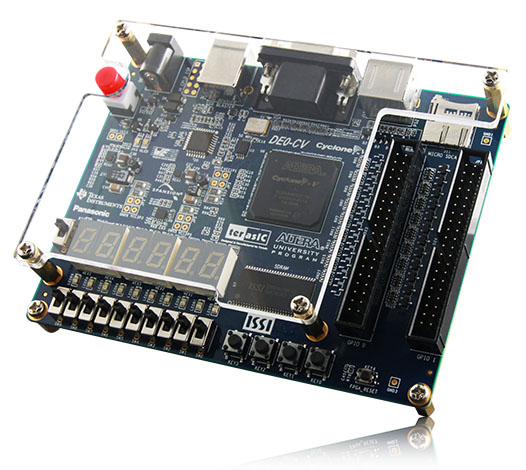
\includegraphics[width=0.45\textwidth, center]{boardimage}
\end{figure}

\pagebreak

\tableofcontents
\thispagestyle{empty}
\pagebreak



\section {Introduction}
	\subsection {Google Test}
	\tab Google Test is a unit testing library for the C++ programming language, based on the xUnit architecture. This section describes some good reasons why we decided to use this framework.
	\begin{itemize}
		\item Google Test is designed to be portable and it works around various bugs in various compilers and environments
		\item Google's test framework has built-in assertions that are deployable in software where exception handling is disabled
		\item Running the tests is simple and it’s easy to write assertions that generate informative messages
		\item Google Test automatically detects your tests and doesn’t require you to enumerate them in order to run them.
		\item Google's test framework provides excellent support for handling such situations. You can repeat the same test a lot of times using the Google framework
	\end{itemize}
	
	\subsection {gcov - coverage testing tool}
	\tab gcov is a test coverage program. We used it in concert with GCC to analyze our programs to help create more efficient, faster running code and to discover untested parts of your program. We used gcov as a profiling tool to help discover where our optimization efforts will best affect our code.


\section {Convolution Layer}
	\subsection {Convolution}
	\tab The convolutional layer is one of the most important layer, since the alexnet architecture is a CNN (Convolutional Neural Network) basically. It contains five layers of this type, thus the convolution function should be carefully implemented and tested.
	The idea is to go through all image pixels and use the filter on them. However the filter might not cover the right pixels that's why we need to check in every iteration if the latter is within the image. Other important things to be considered in this procedure. For instance the caffe model of the layer itself, which provide further specification other than usual channels, height and width.
	
	\subsection {ReLU}
	\tab The caffe model suggest also that the activation function should be considered as a layer too. In order to achieve this approach, we just pass the output of the convolutional as an input for this layer. The function will be applied on the image data and the dimensions of the output do not changes.

	\subsection {Test}
	\tab In order to avoid any unexpected behaviour of the convolutional layer we apply different filters with diffrerent strides on the input. Differents paddings were also used by the input. However we model the image as a set of data and do not use real images
in this approach, so that we can avoid interpreting graphical representation by the output. The data are represented as vectors of float. The expected output are calculated manually and compared to the one produced by the layer. See \ref{fig:figureName}

\section {Fully Connected Layer}
	\subsection {fully Connected}
	\tab This layer basically takes an input volume (whatever the output is of the conv or ReLU or pool layer preceding it) and outputs an N dimensional vector where N is the number of classes that the program has to choose from.

	\subsection {Test}
	\tab TEST(fully\_connected\_layer, test\_fully\_connected\_layer): for this test we have created this objects:
	\begin {itemize}
		\item Weights: object of an Image
		\item fully\_connected\_layer: object of Fully Connected Layer class
		\item inputImage: input image
		\item expectedOutput: expected output
		\item outputFrom\_Fully\_connected\_layer: output of the fully connected layer for the input image
	\end {itemize}
\tab After creating this objets and adding the data to each object we tested if the expected output is equals to the output of the connected layer with (ASSERT\_EQ)


\end{document}